%************************************************
\chapter{Platform Specific Functionality}\label{ch:ui}
%************************************************

Thanks to the framework we chose to use, and the desire to present our application as natively as possible, there exists the need for some platform specific functionality. Most of this functionality has to do with the \ac{UI} and some third-party libraries.

This chapter will be divided in two parts, one for iOS and one for Android. In here we will also discuss all about the \texttt{callback} functions we mentioned earlier. 

\section{Android UI}

The main reason we chose \textit{Xamarin} as the framework for the development of our application is the fact that we can develop the \ac{UI} in a completely independent fashion.

On the Android side of things, this means using specially crafted \ac{XML} files for defining the look of the application. Under Xamarin Studio, we have two options for laying out the content of each view:  We can use the Android Layout Editor to drag and drop elements from a toolbox or we can  directly edit the \ac{XML} source code and change everything manually.

Since most of the application is composed of Lists and Grids, it is actually easier to manually edit the \ac{XML} source code, than to mess around with the visual editor.

\autoref{list:and_xml} and \autoref{fig:and_layout} show both sides of the same file, the source and how it looks inside the Android Layout Editor.

Describing what each element inside the \ac{XML} file is, how they work and why they work that way is outside the scope of this work. If you need more information about the inner workings of the Android Operating System, please refer to more specific literature.


\lstset{language=XML}
\begin{lstlisting}[frame=lt,caption=Company.axml, label={list:and_xml}]
<?xml version="1.0" encoding="utf-8"?>
<LinearLayout xmlns:android="http://schemas.android.com/apk/res/android"
    android:orientation="vertical"
    android:layout_width="wrap_content"
    android:layout_height="wrap_content">
    <ImageView
        android:src="@android:drawable/ic_menu_gallery"
        android:layout_width="match_parent"
        android:layout_height="match_parent"
        android:padding="5dip"
        android:gravity="center"
        android:id="@+id/company_image" />
    <TextView
        android:id="@+id/Name"
        android:layout_width="match_parent"
        android:layout_height="wrap_content"
        android:ellipsize="end"
        android:singleLine="true"
        android:textAppearance="?android:attr/textAppearanceSmall"
        android:padding="5dip"
        android:gravity="center"
        android:text="Test" />
</LinearLayout>
\end{lstlisting}


\begin{figure}[H]
    \begin{center}
        {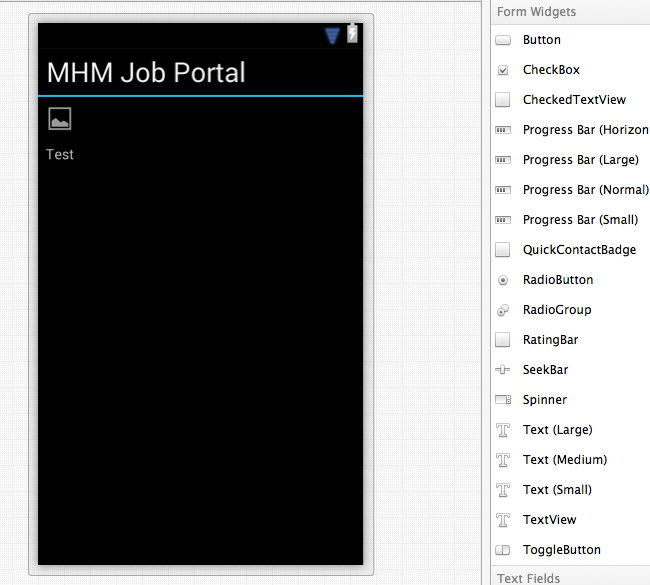
\includegraphics[width=0.75\linewidth]{gfx/and_view}}
        \caption[Android Layout Editor]{Android Layout Editor}\label{fig:and_layout}
    \end{center}
\end{figure}

\subsection{Views, Items and Adapters}
Our Job Portal Aggregator consists of information that is easily packable inside a list, this is why the main view of the application consists of a list of the latest vacancies available.

In order to display this information we need to define a view group where the information will be placed and a view item that represents each element inside the list. All these is done inside the \ac{XML} layout files.

\begin{lstlisting}[frame=lt,caption=Publication.axml, label={list:pub_xml}]
<?xml version="1.0" encoding="utf-8"?>
<LinearLayout xmlns:android="http://schemas.android.com/apk/res/android"
    android:orientation="horizontal"
    android:layout_width="fill_parent"
    android:layout_height="fill_parent">
    <ImageView
        android:src="@android:drawable/ic_menu_gallery"
        android:layout_width="57.2dp"
        android:layout_height="63.0dp"
        android:id="@+id/company_image" />
    <LinearLayout
        android:orientation="vertical"
        android:layout_width="fill_parent"
        android:layout_height="fill_parent">
        <TextView
            android:id="@+id/Title"
            android:layout_width="match_parent"
            android:layout_height="wrap_content"
            android:ellipsize="end"
            android:singleLine="true"
            android:textAppearance="?android:attr/textAppearanceMedium"
            android:padding="5dip"
            android:text="Test" />
        <TextView
            android:id="@+id/Description"
            android:layout_width="match_parent"
            android:layout_height="wrap_content"
            android:padding="5dip"
            android:text="Test" />
    </LinearLayout>
</LinearLayout>
\end{lstlisting}

\autoref{list:pub_xml} describes a Publication element and defines how it will be shown inside the main list. It features the company logo (\texttt{<ImageView>}), the Publication's Title just to the right of the image and its Short Description just bellow the title.

But this is just for one item, we need to define the list that will hold a collection of Publications. In \autoref{list:pubList_xml} we can see that all that is needed is a \texttt{ListView} item. 

\begin{lstlisting}[frame=lt,caption=PublicationsList.axml, label={list:pubList_xml}]
<?xml version="1.0" encoding="utf-8"?>
<LinearLayout xmlns:android="http://schemas.android.com/apk/res/android"
    android:id="@+id/pub_list"
    android:orientation="vertical"
    android:layout_width="fill_parent"
    android:layout_height="fill_parent">
    <ListView
        android:id="@+id/Publications"
        android:layout_width="match_parent"
        android:layout_height="wrap_content" />
</LinearLayout>
\end{lstlisting}

Now that we have defined the list and the appearance of each item within it, we need to connect these elements with real data. That's where adapters come into play. 

\texttt{Adapters} are in charge of populating the list using a collection of items that gets passed via the class constructor. They implement a \texttt{GetView} method that matches elements from the actual object to its visual representation inside the list and define some simple methods for member data accessibility.

\lstset{language=[Sharp]C}

\begin{lstlisting}[frame=lt,caption=PublicationsListAdapter.cs, label={list:pubList_cs}]
class PublicationsListAdapter : BaseAdapter<Publication> {
	readonly LayoutInflater _context; 
	public IList<Publication> Publications { get; set; }
	public PublicationsListAdapter (LayoutInflater context, IList<Publication> publications) {
		_context = context;
		Publications = publications;		
	}
	public override View GetView(int position, View convertView, ViewGroup parent) {
		var view = convertView ?? _context.Inflate(Resource.Layout.Publication, null);
		var pub = Publications[position];
		var db = DatabaseHelper.Instance.Connection;
		var company = db.Table<Company> ().Where (c => c.Name.Equals(pub.Company)).First();
		var imgFile = new File (company.IconPath);
		Bitmap imgBitmap = BitmapFactory.DecodeFile(imgFile.AbsolutePath);
		view.FindViewById<TextView>(Resource.Id.Title).Text = pub.Title; 
		view.FindViewById<TextView> (Resource.Id.Description).Text = pub.ShortDescription;
		view.FindViewById<ImageView> (Resource.Id.company_image).SetImageBitmap (imgBitmap);
		return view; 
	}
}
\end{lstlisting}

Another possibility for displaying a cluster of data is called Grids. They allow you to neatly pack data into what can be considered a two-dimensional list. We use Grids in our application to display the available companies that offer vacant positions.

Grids behave almost identically to Lists. They need an Item Definition, an Adapter and the Grid Definition itself. There is no distinction between adapters and item definitions for lists and their counterparts for grids. The only difference is in how the collections are laid out.

\lstset{language=XML}
\begin{lstlisting}[frame=lt,caption=CompaniesGrid.axml, label={list:grid_xml}]
<GridView xmlns:android="http://schemas.android.com/apk/res/android"
    android:id="@+id/Companies"
    android:layout_width="fill_parent"
    android:layout_height="fill_parent"
    android:columnWidth="120dp"
    android:numColumns="auto_fit"
    android:verticalSpacing="10dp"
    android:horizontalSpacing="10dp"
    android:stretchMode="columnWidth"
    android:gravity="center" />
\end{lstlisting}

This means that the \texttt{CompaniesAdapter} looks exactly the same as the \texttt{PublicationsAdapter}, with the small difference that the collection used is for \texttt{Company} objects. And the \texttt{Company} item has one \texttt{<TextView>} less, because it only needs one for the Company name.
\vfill

\subsection{Activities, Fragments and Navigation}

With the views, items and adapters we have everything necessary to format and display our data just how we want it, but we still need something to call the views and manage their life cycle. That's where activities and fragments come in. They are in charge of actually displaying the views to the user and handling interaction.

To make navigation simpler, we utilize Android's own Navigation Drawer that swipes from the left side or appears when the Action Bar is clicked. In order to fully take advantage of this feature it is necessary to implement each view manager as a fragment within a main activity that handles them. Let's describe each fragment before handling the main activity.

Each fragment takes care of preparing the view, displaying it when it's time, and what happens when the user clicks on an item. 

The \texttt{PublicationsFragment} serves different purposes based on the context form where it's being called. It serves as the main view getting filled with the latest publications and also as a filtered view, containing only the right publications.

\lstset{language=[Sharp]C}

\begin{lstlisting}[frame=lt,caption=PublicationsFragment.cs, label={list:pub_frag}]
public class PublicationsFragment : Fragment {
	[...]
	public PublicationsFragment (bool remoteLoad = true, int companyId = 0) {
		_reload = remoteLoad;
		_companyId = companyId;		
	}
	[...]
	
	public override View OnCreateView (LayoutInflater inflater, ViewGroup container, Bundle savedInstanceState) {
		parser = new PublicationsParser ();
		dbHelper = DatabaseHelper.Instance.Connection;
		_inflater = inflater;
		var cnHelper = ConnectivityHelper.Instance (Activity);
		layout = inflater.Inflate(Resource.Layout.PublicationsList, container, false);
		publicationsList = layout.FindViewById<ListView> (Resource.Id.Publications);
		if (_reload) {
			if (cnHelper.NetworkAvailable ()) {
				parser.UpdatePublications (publications => Activity.RunOnUiThread (() => {
					publicationsList.Adapter = new PublicationsListAdapter (_inflater, publications);
					publicationsList.ItemClick += (sender, e) => {
						[...]
						StartActivity(intent);
					};
				}));
			} else {
				SetupTable (_companyId);
			}		
		} else {
			SetupTable (_companyId);	
		}
		return layout;
	}
}
\end{lstlisting}

Once the Fragment gets called into view, it launches the \texttt{OnCreateView} method that is in charge of setting up the entire list. Depending on the context, it checks for a network connection and prepares the table based on the response. If it should reload the table and there is a connection available, it calls the \texttt{UpdatePublications} method from the \texttt{PublicationsParser} and works with the returned data, otherwise it calls the local \texttt{SetupTable} method.

\begin{lstlisting}[frame=lt,caption=SetupTable, label={list:pub_setup}]
public void SetupTable (int companyId) {
	IList<Publication> publications;
	if (companyId == 0) {
		publications = parser.Publications;
	} else {
		var company = dbHelper.Get<Company> (companyId);
		publications = dbHelper.Table<Publication> ().Where (p => p.Company.Equals (company.Name)).ToList ();
	}
	var adapt = new PublicationsListAdapter (_inflater, publications); 
	publicationsList.Adapter = adapter;
	publicationsList.ItemClick += (sender, e) => {
		var pub = adapt.Publications[e.Position];
		var intent = new Intent (Activity, typeof(PublicationActivity));
		intent.PutExtra ("pub_id", pub.Id);
		StartActivity (intent);
	};
}
\end{lstlisting}


The \texttt{SetupTable} method takes care of populating the list with the required data. If \texttt{\_companyId} is set to a value other than 0, it populates the list with Publications belonging only to the Company with a matching ID, if it's set to 0, it loads all Publications from the database.

In here, just like on the \texttt{OnCreateView} method, we set what happens when the user clicks on an item of the list. We do this by setting the \texttt{ItemClick} listener. This listeners gets the position of the item that was clicked, and with this index, it fetches a \texttt{Publication} object from the Adapter. Once it has the object it prepares an \texttt{Intent} in order to start a new \texttt{Activity}. In the intent we can save extra information and pass this information to the new Activity. By doing this we can tell the \texttt{PublicationActivity} what ID the clicked Publication has.\\
\newline
The \texttt{CompaniesFragment} behaves in pretty much the same way. It fetches the grid from the \ac{XML} file, sets the adapter and passes to it a collection of companies. Once the Grid is ready to be displayed, we set the click handler. This click handler gets the ID of the Company that was clicked and prepares a \texttt{PublicationsFragment} to show only the Publications belonging to this Company by setting the \texttt{companyID} parameter. Once the item is clicked, the current fragment gets replaced by the newly created \texttt{PublicationsFragment}.\\


\begin{lstlisting}[frame=lt,caption=CompaniesFragment.cs, label={list:comp_frag}]
public class CompaniesFragment : Fragment
{
	public override void OnCreate (Bundle savedInstanceState)
	{
		base.OnCreate (savedInstanceState);
		Activity.SetTitle (Resource.String.companies);
		SetHasOptionsMenu (true);
	}

	public override View OnCreateView (LayoutInflater inflater, ViewGroup container, Bundle savedInstanceState)
	{
		var parser = new CompaniesParser ();
		var companies = parser.Companies;
		var layout = inflater.Inflate(Resource.Layout.CompaniesGrid, container, false);
		var companiesGrid = layout.FindViewById<GridView> (Resource.Id.Companies);
		companiesGrid.Adapter = new CompaniesAdapter (inflater, companies);
		companiesGrid.ItemClick += (sender, e) => {
			var comp = companies [e.Position];
			var publications = new PublicationsFragment (false, comp.Id);
			MainActivity.mDrawerToggle.DrawerIndicatorEnabled = false;
			FragmentManager.BeginTransaction ().Replace (Resource.Id.content_frame, publications).AddToBackStack (null).Commit ();
		};
		return layout;
	}
}
\end{lstlisting}



The next step after this is to show a detailed view of the Publication the user chose. This is handled by the \texttt{PublicationActivity}. This activity has its own layout describing the elements that will be presented to the user. It supports separate \texttt{TextViews} for all of the information that needs to be displayed about this position and different \texttt{ImageViews} for the logo of the company and any other visual information that might be relevant to this particular Publication.

It also features a \textit{Share} button that the user can use to share a direct link to this Publication with his friends via \textit{Twitter}, \textit{Facebook}, \textit{SMS} or any other application that can handle an HTTP link.\newline

But all of components would never be shown if it weren't for the \texttt{MainActivity}. This activity is in charge of creating the navigation drawer, managing the fragments and even handling search events.

The \texttt{MainActivity} uses a special kind of layout that contains the Navigation Drawer, a special \texttt{ListView} that will hold the navigation items and a \texttt{FrameLayout} where the different fragments will be placed, all inside a special layout format called \texttt{DrawerLayout}. And the \texttt{OnCreate} method is where everything gets defined.
\newpage

\begin{lstlisting}[frame=lt,caption=MainActivity.cs, label={list:main_ac2}]
protected override void OnCreate (Bundle bundle) {
	base.OnCreate (bundle);
	SetContentView (Resource.Layout.Navigation);
	cnHelper = ConnectivityHelper.Instance (this);
	mDrawerLayout = FindViewById<DrawerLayout> (Resource.Id.drawer_layout);
	mDrawerList = FindViewById<ListView> (Resource.Id.left_drawer);
	mDrawerList.Adapter = new DrawerAdapter (this);
	mDrawerList.ItemClick += (sender, e) => {
		switch (e.Position) {
		case 0:
			var publications = new PublicationsFragment (false);
			FragmentManager.BeginTransaction ().Replace (Resource.Id.content_frame, publications).Commit ();
			SetTitle (Resource.String.main_title);
			mDrawerLayout.CloseDrawer (mDrawerList);
			break;
		case 1:
			var companies = new CompaniesFragment ();
			FragmentManager.BeginTransaction ().Replace (Resource.Id.content_frame, companies).Commit ();
			SetTitle (Resource.String.companies);
			mDrawerLayout.CloseDrawer (mDrawerList);
			break;
		} 
	};
	mDrawerLayout.SetDrawerShadow (Resource.Drawable.drawer_shadow, GravityCompat.Start);
	mDrawerToggle = new ActionBarDrawerToggle (this, mDrawerLayout, Resource.Drawable.ic_drawer, Resource.String.drawer_open, Resource.String.drawer_close);
	mDrawerLayout.SetDrawerListener (mDrawerToggle);
	var pubs = new PublicationsFragment ();
	FragmentManager.BeginTransaction().Replace(Resource.Id.content_frame, pubs).Commit();
	HandleIntent (Intent);
}
\end{lstlisting}
\vfill

As always, we set the layout for the activity to point to the Navigation layout and get references to the objects inside the layout, like the navigation list (\texttt{mDrawerList}). We then populate the list with a special \texttt{DrawerAdapter} that contains the menu items and set what happens when the user clicks an item.

Depending on the position of the click, we either replace the current fragment with a \texttt{PublicationsFragment} or a \texttt{CompaniesFragment}, set the title of the Activity to match the current fragment and close the navigation drawer.

Next we continue to set up the navigation drawer in order for it to work properly, not only by clicking the Action Bar, but also by swiping from the left side of the screen, then we need to insert a \texttt{PublicationFragment} into the activity, otherwise it has no content.

And finally we check if there is an Intent that needs to be handled appropriately. This is specially necessary for search intents, which we will discuss later on.




\section{Android Functionality}

Thanks to the difference between Android and iOS, there are some aspects of the application that need to be implemented separately for each platform. We already saw this happen with the \ac{UI} elements, but there is also some core functionality that needs the same treatment.

\subsection{Callback Functions}\label{callback:and}

The \textit{Callback Functions} are anonymous, platform specific methods that are passed to the generic data handling code, in order to be executed when the data is ready.

We already saw where the \texttt{callback} functions are executed in \autoref{list:db-pubparse} and \autoref{list:search}, which are part of the \texttt{PublicationsParser} file, and an example of one in \autoref{list:pub_frag}. We will now take a closer look and see how they actually do what they do.

\begin{lstlisting}[frame=lt,caption=Callback, label={list:call_and}]
parser.UpdatePublications (publications => Activity.RunOnUiThread (() => {
	var adapter = new PublicationsListAdapter (_inflater, publications);
	publicationsList.Adapter = adapter;
	publicationsList.ItemClick += (sender, e) => {
		var pub = adapter.Publications [e.Position];
		var intent = new Intent(Activity, typeof(PublicationActivity));
		intent.PutExtra("pub_id", pub.Id);
		StartActivity(intent);
	};
}));
\end{lstlisting}

The callback function is everything that is between the parenthesis after the \texttt{UpdatePublications} method call. It consists of a parameter declaration (\texttt{publications}) followed by a lambda operator. Everything after this operator is what actually gets executed. 

Since all the data fetching methods run in the background, we need to specify that our code needs to run in the same thread as the \ac{UI}, otherwise we can't manipulate anything that is on the view. So we open a \texttt{RunOnUiThread} call and place our logic in here.

This logic is pretty straight-forward. We prepare an adapter for the \texttt{PublicationsList} with the parameter that got passed when the callback method was activated. In this case it is a collection of Publications. Then we set the adapter and declare what happens when the user clicks on an item, something that we discussed previously.

The best thing about this type of anonymous functions, it that it allows us to write code that doesn't care about the specific implementation of something, but rather focuses on executing it, we then leave the implementation to the specific platform.



\subsection{Search}

Thanks to the \textit{ActionBar}, there is no need for a separate activity or fragment to handle the search functionality. It is all done right in the Activity that will show the search icon. For us, this is the \texttt{MainActivity}.

For an activity to be able to handle searches, it needs to declare this functionality in the \texttt{AndroidManifest.xml} file. Thanks to \textit{Xamarin}, there is no need to manually edit the manifest, it is all done right inside the activity file itself. 

Take a look at \autoref{list:main_ac}, it shows what is necessary for the activity to be able to handle incoming search requests. All the attributes before the class opener take care of creating the right entries in the Manifest file. In here we define an \texttt{IntentFilter} for the \texttt{ActionSearch} action, this tells Android, that this Activity will handle every action that is started with the intention to perform a search.
\vfill
\begin{lstlisting}[frame=lt,caption=MainActivity.cs, label={list:main_ac}]
[Activity (Label = "Latest Jobs", Theme = "@android:style/Theme.Holo.Light", LaunchMode = LaunchMode.SingleTop)]
[IntentFilter (new [] { Intent.ActionSearch })]
[MetaData (("android.app.searchable"), Resource = "@xml/searchable")]
public class MainActivity : Activity {
	[...]
	void HandleIntent (Intent intent) {
		if (Intent.ActionSearch.Equals(intent.Action)){
		var query = intent.GetStringExtra (SearchManager.Query);
		var parser = new PublicationsParser ();
		SetTitle (Resource.String.search_results);
		mDrawerList.SetItemChecked (0, false);
		var publicationsList = FindViewById<ListView> (Resource.Id.Publications);
		if (cnHelper.NetworkAvailable ()) {
		parser.SendSearchParameters (publications => RunOnUiThread (() => {
			var adapter = new PublicationsListAdapter (this.LayoutInflater, publications);
			publicationsList.Adapter = adapter;
			publicationsList.ItemClick += (sender, e) => {
			var pub = adapter.Publications [e.Position];
			var myIntent = new Intent (this, typeof(PublicationActivity));
			myIntent.PutExtra ("remote_id", pub.RemoteId);
			StartActivity (myIntent);
			};
		}), query);				
		} else {
		parser.LocalSearch (publications => RunOnUiThread (() => {
			var adapter = ((PublicationsListAdapter) publicationsList.Adapter);
			adapter.Publications = publications;
			adapter.NotifyDataSetChanged ();
			publicationsList.ItemClick += (sender, e) => {
			var pub = adapter.Publications [e.Position];
			var myIntent = new Intent (this, typeof(PublicationActivity));
			myIntent.PutExtra ("pub_id", pub.Id);
			StartActivity (myIntent);
			};
		}) , query);
		}			
		}		
	}
}\end{lstlisting}

If we need to handle a search, we take a reference to the already loaded list adapter and replace its content with the results given by the search methods. In here we check again for network connectivity and depending on the answer, we either load the results from the local database or from the remote server.  

%\subsection{Third-Party Libraries}

%To display some alerts with style, we use a library called \textit{AndHUD}. This library generates alerts, progress bars and notifications with a Heads Up Display Style.
%
%\begin{figure}[H]
%    \begin{center}
%        {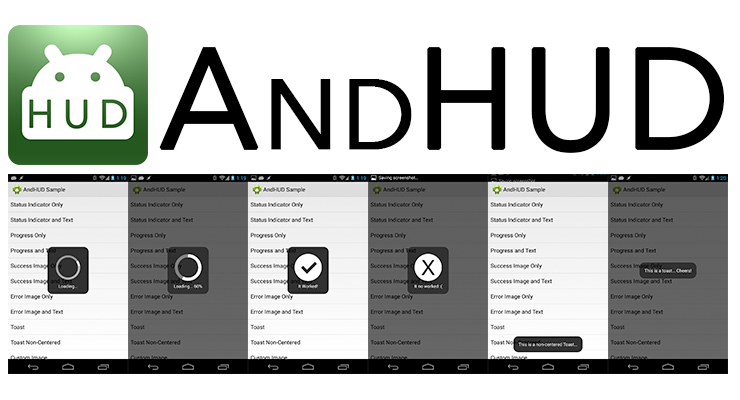
\includegraphics[width=0.70\linewidth]{gfx/andhud}}
%        \caption[AndHUD]{AndHUD}
%    \end{center}
%\end{figure}

%To simplify some user interaction we use a library called \textit{PullToRefreSharp}. This library allows use to modify a normal list view, so that it can be refreshed by pulling the list down and releasing it.
%
%\begin{figure}[H]
%    \begin{center}
%        {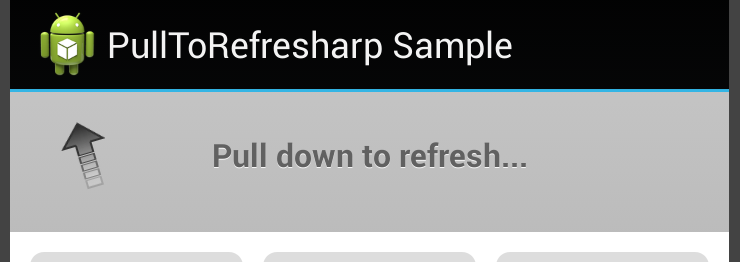
\includegraphics[width=0.65\linewidth]{gfx/pulltr}}
%        \caption[PullToRefreSharp]{PullToRefreSharp\footnotemark}
%    \end{center}
%\end{figure}
%\footnotetext{Source: \url{http://components.xamarin.com/resources/icons/component-255/slide1.png}}



%%%%%%%%%%%%%%%%%%%%%%%%%%%%%%%%%%%%%%%%%%%%%%%%%%%%%%%%%%%%%%%%%%%%%%%%%%

\section{iOS UI}

Now that we discussed in detail every Android component, it is iOS' turn. There is a very big difference in how both platforms handle the \ac{UI} design. iOS also has an interface designer that lets you visually add elements to the layout, but unlike Android, you cannot edit the source code generated by the designer and you need to manually bind each element in the designer to the backend code, before you can use them. Android lets you access these items programmatically without the need for a manual bind.

This added complexity gets compensated by the fact that simple components like tables don't need a layout file, they can be generated entirely by code.

As an example of the Xcode View Editor we can take a look at \autoref{fig:xcode}. It shows how we define the look of a cell for the Companies Collection and how we need to link the elements into the code, so that we can use them in \textit{Xamarin Studio}.

\begin{figure}[H]
    \begin{center}
        {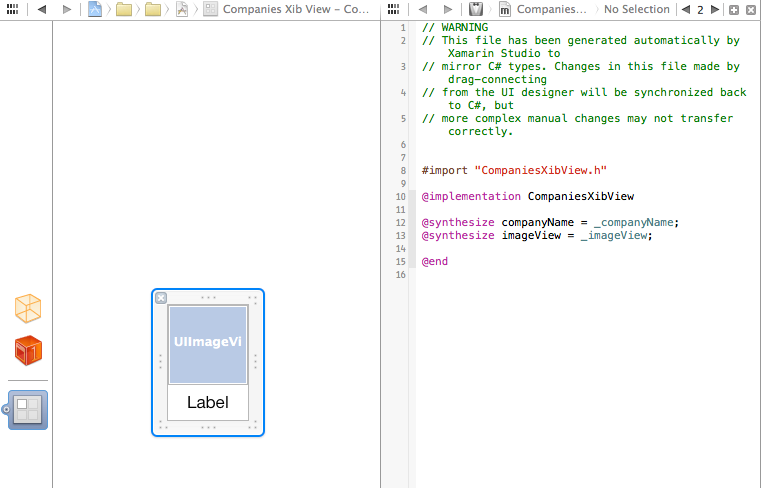
\includegraphics[width=1\linewidth]{gfx/xcode}}
        \caption[Xcode View Editor]{Xcode View Editor}
        \label{fig:xcode}
    \end{center}
\end{figure}

And, once again, going into every detail of the inner workings of iOS and how they translate to \textit{Xamarin's} own implementation is beyond the scope of this work. If you need more detailed information about this topic, please refer to more specific literature.

\subsection{Controllers, Sources and Navigation}

In order to have a similar navigation scheme as in Android with the Navigation Drawer, we need to use a third-party library called \texttt{SlideoutNavigation}. 

This library modifies the normal \texttt{UINavigationController} that is built in into iOS and adds an extra \texttt{ViewController} that can appear from every side of the screen. For our application we just need a view that swipes from the left side of the screen containing a list of menu entries.

\begin{lstlisting}[frame=lt,caption=LeftMenu.cs, label={list:ios_menu}]
public class LeftMenu : DialogViewController {
	public LeftMenu () : base (UITableViewStyle.Plain, null) {
		var CompaniesLayout = new CompaniesLayout ();
		Root = new RootElement ("Menu") {
			new Section () {
				new BadgeElement (UIImage.FromBundle ("Images/ic_home.png"), "Home".t(), () => NavigationController.PushViewController (new PublicationsViewController (true, true), true)),
				new BadgeElement (UIImage.FromBundle ("Images/ic_companies.png"), "Companies".t(), () => NavigationController.PushViewController (new CompaniesViewController (CompaniesLayout), true)),
				new BadgeElement (UIImage.FromBundle ("Images/ic_search.png"), "Search".t(), () => NavigationController.PushViewController (new SearchViewController (), true))
			}
		};
	}
}
\end{lstlisting}

\autoref{list:ios_menu} shows us the \texttt{ViewController} that will be displayed when the user clicks on the menu button or swipes the screen from the left. To create the menu, we use a \texttt{DialogViewController} class. The special thing about this class is that it doesn't exist in \marginpar{Cocoa is the windowing library for iOS and Mac} Objective-C or Cocoa. This class was created by the developers of \textit{Xamarin} and \textit{MonoTouch} in order to simplify the creation of views with different and complex elements.

Unlike Android, there is no Main Activity or Main Controller to manage everything inside the application, every view that needs to be displayed is loaded from the menu and pushed on top of the navigation stack. There is however an \texttt{AppDelegate} file that is in charge of launching the application and setting the navigation controllers.

\begin{lstlisting}[frame=lt,caption=AppDelegate.cs, label={list:app_delegate}]
[Register ("AppDelegate")]
public class AppDelegate : UIApplicationDelegate {
	public SlideoutNavigationController Menu { get; private set; }
	UIWindow window;
	public override bool FinishedLaunching (UIApplication application, NSDictionary launchOptions) {
		window = new UIWindow (UIScreen.MainScreen.Bounds);
		Menu = new SlideoutNavigationController ();
		Menu.TopView = new PublicationsViewController (false);
		Menu.LeftMenuButtonText = "Menu";
		Menu.MenuViewLeft = new LeftMenu ();
		window.RootViewController = Menu;
		window.MakeKeyAndVisible ();			
		return true;
	}
}
\end{lstlisting}

The Top View, meaning the first view of the application, is, just like with Android, a view containing the latest Publications. This view is managed by the \texttt{PublicationsViewController}. Since this is a simple table view, it doesn't need a layout and can be set up completely with code.

\begin{lstlisting}[frame=lt,caption= PublicationsViewController.cs, label={list:ios_pub_cont}]
public class PublicationsViewController : UITableViewController	{
	bool _fromMenu = false;
	readonly PublicationsParser _parser;
	public PublicationsViewController (bool fromMenu = false) : base (UITableViewStyle.Plain) {
		_parser = new PublicationsParser ();
		_fromMenu = fromMenu;
	}
	public override void ViewDidLoad ()	{
		base.ViewDidLoad ();
		Title = "LatestJobTitle".t();
		TableView.BackgroundColor = UIColor.FromWhiteAlpha(0.95f, 1.0f);
		RefreshControl = new UIRefreshControl ();
		RefreshControl.ValueChanged += (sender, e) => RefreshTable ();
	}
	public void RefreshTable(UIAlertView loading = null) {		if (NetworkAvailable ()) {
			_parser.UpdatePublications(publications => InvokeOnMainThread (() => {
				TableView.Source = new PublicationsViewSource (publications, NavigationController);
				TableView.ReloadData ();
				if (loading != null)
					loading.DismissWithClickedButtonIndex (0, true);
			}));			
		} else {
			var publications = _parser.Publications;
			TableView.Source = new PublicationsViewSource (publications, NavigationController);
			TableView.ReloadData ();
			if (loading != null)
				loading.DismissWithClickedButtonIndex (0, true);
		}
		RefreshControl.EndRefreshing ();
	}
}
\end{lstlisting}

A great benefit of iOS is that it doesn't need an extra library to implement "Pull to Refresh". Since iOS 5.0 any \texttt{TableView} comes with the ability to define an \texttt{RefreshControl} that will execute an action when the table is pulled down.

Almost in the same way as Android, we need an extra class for the actual elements of the list. Within iOS it is called a \texttt{ViewSource} and it is here where we define what happens when a user clicks on an element of the table.

\begin{lstlisting}[frame=lt,caption= PublicationsViewSource.cs, label={list:pub_source}]
public class PublicationsViewSource : UITableViewSource	{
	readonly IList<Publication> _publications; 
	readonly UINavigationController _controller;
	readonly SQLiteConnection _db;
	public PublicationsViewSource (IList<Publication> publications, UINavigationController controller) {
		_publications = publications;
		_controller = controller;
		_db = DatabaseHelper.Instance.Connection;
	}
	public override int RowsInSection (UITableView tableview, int section) {
		return _publications.Count;;
	}
	public override UITableViewCell GetCell (UITableView tableView, NSIndexPath indexPath) {
		var cell = tableView.DequeueReusableCell (PublicationsViewCell.Key) as PublicationsViewCell ?? new PublicationsViewCell ();
		var publication = _publications[indexPath.Row];
		cell.TextLabel.Text = publication.Title;
		var company = _db.Table<Company> ().Where (c => c.Name.Equals (publication.Company)).First ();
		cell.ImageView.Image = UIImage.FromFile (company.IconPath);
		cell.DetailTextLabel.Text = publication.ShortDescription;
		return cell;
	}
	public override void RowSelected(UITableView tableView, NSIndexPath indexPath) {
		_controller.PushViewController (new PublicationViewController (_publications[indexPath.Row]), true);
	}
}
\end{lstlisting}

The \texttt{RowSelected} method inside \autoref{list:pub_source} handles what happens when a user clicks a row. We fetch the selected Publication and pass it to a new \texttt{ViewController} that will be pushed into the navigation stack.

This \texttt{PublicationViewController} then displays detailed information about the Publication in the same manner as the \texttt{PublicationActivty} on the Android side.\newline

The second part of the application is a \texttt{ViewController} containing the available Companies that have open job positions. Just like in Android, these companies are organized in a grid that under iOS is called a Collection.

A \texttt{CollectionView} consists of a \texttt{CollectionViewCell}, a \texttt{XIB} file containing its layout definition and a Controller that handles clicks and sets up the \ac{UI}. We already saw this exact \texttt{XIB} file at the beginning of this section in \autoref{fig:xcode}.

The content of the collection is filled at the same time as the collection is created, and when the user clicks on an item of the collection, the Publications get filtered by reusing the \texttt{PublicationsViewController} and its \texttt{ViewSource}, in a similar way as with Android.
 

\section{iOS Functionality}

As mentioned before, there are some aspects of the application that need to be implemented separately for each platform. We already saw this happen with the \ac{UI} elements, but some core functionality also needs special attention.

\subsection{Callback Functions}\label{callback:ios}

We already described what \textit{Callback Functions} are, how they work and why they are helpful to us. All that's left is to see how they operate inside iOS.

\begin{lstlisting}[frame=lt,caption=Callback iOS, label={list:call_ios}]
parser.UpdatePublications(publications => InvokeOnMainThread (() => {
	TableView.Source = new PublicationsViewSource (publications, this, _db);
	TableView.ReloadData ();
}));
\end{lstlisting}

The code is exactly the same in functionality, but looks somewhat different. We populate the table source with the \texttt{publications} passed by the calling method and set this as the source for the main table, we then just need reload the data. Unlike Android, the click handlers are done inside the source definition for the table. 


\subsection{Search}

Unlike Android, we need a separate ViewController to handle the searches. This view is accessible from the navigation menu and is empty upon call. It gets loaded with results as soon as the user begins typing something in the search bar.

\begin{lstlisting}[frame=lt,caption=SearchViewController.cs, label={list:ios_search}]
public class SearchViewController : UITableViewController {
	readonly PublicationsParser _parser;
	readonly SQLiteConnection _db;
	readonly UISearchBar searchBar;
	public SearchViewController (SQLiteConnection db) : base (UITableViewStyle.Grouped) {
		[...]
	}
	public override void ViewDidLoad ()	{
		base.ViewDidLoad ();
		searchBar.SizeToFit ();
		Title = "Search".t ();
		TableView.TableHeaderView = searchBar;
		searchBar.SearchButtonClicked += (s, e) => searchBar.ResignFirstResponder ();
		searchBar.TextChanged += (s, e) => RefineSearchItems ();
	}
	protected void RefineSearchItems() {
		if (searchBar.Text == "") {
			TableView.Source = null;
			TableView.ReloadData ();
		} else {
			if (PublicationsViewController.NetworkAvailable ()) {
				_parser.SendSearchParameters (publications => InvokeOnMainThread (() => {
					TableView.Source = new PublicationsViewSource (publications, NavigationController, _db);
					TableView.ReloadData ();
				}), searchBar.Text);
			} else {
				_parser.LocalSearch (publications => InvokeOnMainThread (() => {
					TableView.Source = new PublicationsViewSource (publications, NavigationController, _db);
					TableView.ReloadData ();
				}), searchBar.Text);
			}			
		}			
	}
}
\end{lstlisting}

As we saw with Android, depending on the connection state, the results are either loaded from the local database or from the remote server.

\subsection{Third-Party Libraries}

Like we mentioned earlier, we need a library called \textit{SlideoutNavigation} in order implement a similar navigation style in iOS as we have for Android with the Navigation Drawer. It performs in pretty much the same way as the Navigation Drawer, if we use a List element to save the different menu options.

%%%%%%%%%%%%%%%%%%%%%%%%%%%%%%%%%%%%%%%%%%%%%%%%%%%%%%%%%%%%%%%%%
\section{Final Thoughts}
It is amazing how, even in the platform specific implementation, we can find similarities. If it weren't for \textit{Xamarin} the code and effort necessary to accomplish this application on both platforms would be orders of magnitude bigger.

\textit{Xamarin} allowed us not only to share code, but also to share a programming language, making it even simpler to jump into both platforms. The ease of development even makes it easy to port Java or Objective-C code to work with C\#. 